
\documentclass[
  a4paper,
  12pt,
  oneside, % Einseitig bedruckt
  openany, % Kapitel dürfen auf jeder Seite beginnen, nicht nur auf auf der rechten
  final    % final, draft
]{scrreprt}

% Deutsche Silbentrennung
\usepackage[ngerman]{babel}
% Deutsche Umlaute
\usepackage[utf8]{inputenc}
% Verwendung von T1-Schriften (zusätzliche Textsymbole)
%\usepackage[T1]{fontenc}
% Ermöglicht Zugriff auf Textsymbole
\usepackage{textcomp}

% Zeilenabstand
\usepackage{setspace}

% Verbesserter Mathesatz
\usepackage{amsmath}
\usepackage{amsfonts}
\usepackage{amssymb}

% Quellcode-Listings
\usepackage{listings}

% Zum einbinden von Grafiken
\usepackage{graphicx}

% zum festen plazieren von Grafiken
\usepackage{here} 

% Um Abbildungen aus Unterabbildungen zusammenzusetzen
\usepackage{subfig}

% BibTex
\usepackage{bibgerm}

% Literaturstyle
\bibliographystyle{geralpha}

\usepackage{color}							% Farbendefinitionen
\definecolor{mygray}{gray}{.85} % Graue Farbe definieren
\definecolor{mygreen}{rgb}{.1,.5,.2} % Dunkelgrüne Farbe definieren

\lstset{												% Definieren des Quellcodes
		language=c++,
		numbers=left,
		showstringspaces=false,
		breaklines=true,
		numbers=left,
		numberstyle=\small,
		backgroundcolor={\color{mygray}},
		basicstyle=\sffamily\scriptsize,
		keywordstyle={\color{blue}\bfseries},
		commentstyle={\color{mygreen}\slshape},
		stringstyle={\color{red}},
		%frame=single
}

% URL-Verlinkung und Metadaten in PDF-Dateien
\usepackage [
  bookmarks=true,         % Show bookmarks bar?
  unicode=false,          % Non-Latin characters in Acrobats bookmarks
  pdftoolbar=true,        % Show Acrobats toolbar?
  pdfmenubar=true,        % Show Acrobats menu?
  pdffitwindow=false,     % Window fit to page when opened
  pdfstartview={XYZ null null 1}, % FitH fits the width of the page to the window
  pdftitle={Algorithmen zur Parallelisierung von DB-Anfragen auf Multi-Core-Prozessoren},    % Title
  pdfauthor={Christian Dirks, Tuan-Si Tran}, % Author
  pdfsubject={Datenmanagement in der Cloud}, % Subject of the document
  pdfcreator={LaTeX},     % Creator of the document
  pdfproducer={Producer}, % Producer of the document
  pdfkeywords={keywords}, % List of keywords
  pdfnewwindow=true,      % Links in new window
  colorlinks=true,        % False: boxed links; true: colored links
  linkcolor=black,        % Color of internal links
  citecolor=black,        % Color of links to bibliography
  filecolor=blue,         % Color of file links
  urlcolor=blue           % Color of external links
 ]{hyperref}
 

\begin{document}

\thispagestyle{plain}
\begin{titlepage}

\center


\includegraphics[width=7cm]{Bilder/h_da_logo}

\vspace{4em}

\Large{
		Hochschule Darmstadt\\
		- Fachbereich Informatik -
}

\vspace{4em}

\large{Datenmanagement in der Cloud}

\vspace{0.5em}

\huge{Algorithmen zur Parallelisierung von DB-Anfragen auf Multi-Core-Prozessoren}

\vspace{2em}

\large
{

\vfill
{
von

%Sortiert nach Nachnamen
Christian Dirks,

Tuan-Si Tran
}

\vfill
{
bei

Prof. Dr. Uta Störl
}
}

\end{titlepage}

% 1.5-facher Zeilenabstand
\onehalfspacing

%\chapter*{Abstract}
\label{sec:Abstract}

In den letzten Jahren wird die Rechenleistung von Computern erhöht, indem Prozessoren mit mehreren Kernen ausgestattet werden. Datenbanksysteme sind allerdings zurzeit noch nicht in der Lage das vollständige Potenzial von Multicore-Prozessoren auszunutzen. In dieser Arbeit behandeln wir vier Algorithmen von verschiedenen Entwicklern, die Datenbanksysteme für Multicore-Architekturen optimieren sollen und vergleichen diese auf Nutzen und Aufwand. Dabei versuchen die Algorithmen sowohl das Caching der Prozessoren als auch Hash-Join und Sort-Operationen so wie die Zugriffspläne für die Nutzung der Mehrkernprozessoren zu verbessern. Es stellt sich dabei heraus, dass alle vier Algorithmen eine signifikante Leistungssteigerung ermöglichen, wobei mit mehr Implementierungsaufwand auch bessere Effekte erzielt werden. Die Algorithmen verbessern eindeutig die Performanz und könnten Einzug in die Datenbanksysteme erhalten.

% Inhaltsverzeichnis
\tableofcontents

% Abbildungsverzeichnis
%\listoffigures
%\addcontentsline{toc}{section}{Abbildungsverzeichnis}

% Tabellenverzeichnis
%\listoftables
%\addcontentsline{toc}{section}{Tabellenverzeichnis}

% Der eigentliche Inhalt
\chapter*{Abstract}
\label{sec:Abstract}

In den letzten Jahren wird die Rechenleistung von Computern erhöht, indem Prozessoren mit mehreren Kernen ausgestattet werden. Datenbanksysteme sind allerdings zurzeit noch nicht in der Lage das vollständige Potenzial von Multicore-Prozessoren auszunutzen. In dieser Arbeit behandeln wir vier Algorithmen von verschiedenen Entwicklern, die Datenbanksysteme für Multicore-Architekturen optimieren sollen und vergleichen diese auf Nutzen und Aufwand. Dabei versuchen die Algorithmen sowohl das Caching der Prozessoren als auch Hash-Join und Sort-Operationen so wie die Zugriffspläne für die Nutzung der Mehrkernprozessoren zu verbessern. Es stellt sich dabei heraus, dass alle vier Algorithmen eine signifikante Leistungssteigerung ermöglichen, wobei mit mehr Implementierungsaufwand auch bessere Effekte erzielt werden. Die Algorithmen verbessern eindeutig die Performanz und könnten Einzug in die Datenbanksysteme erhalten.
\chapter{Einleitung}
\label{sec:Einleitung}
Zugriff auf Speicher ist bisher Bottle-Neck, aber die modernen Ausarbeitrungen zielen auf optimierung der Ausführung durch mehrere CPU-Kerne
Keinen gemeinsamen Speicher.
Moores Gesetz.
Herausforderung - Mehr Kerne ergeben mehr Verwaltungsaufwand

\section{Motivation}
\label{sec:Motivation}
Das Mooresche Gesetz aus den 60iger Jahren sagt aus, dass sich die Zahl der Transistoren auf integrierten Schaltungen alle 18 Monate verdoppelt. Dies wirkt sich auch analog auf die Rechenleistung aus. In den letzten Jahren wird die Erhöhung der Rechenleistung allerdings nicht mehr durch noch schnellere Prozessoren erzielt, sondern durch den Einsatz von mehreren Prozessorkernen, die dann eine Einheit bilden und (echte) parallele Verarbeitung ermöglichen.

Während bei der Verbesserung der Ein-Kern-Prozessoren die Datenbanksysteme ebenso direkt davon profitieren konnten, stellen sich bei Multicore-Prozessoren neue Herausforderungen an das Datenbanksystem. Um das komplette Potential der Multicore-Prozessoren ausreizen zu können, müssen Algorithmen angepasst und neu erfunden werden.

\section{Ziele der Arbeit}
\label{sec:ZieleDerArbeit}
In dieser Arbeit werden verschiedene Ansätze vorgestellt, wie man Datenbanken und deren Algorithmen modifizieren kann, um das volle Potenzial von Multicoreprozessoren auszunutzen. Dabei soll an verschiedenen Punkten angesetzt werden. 

[BILD Layout]

Optimierungen können Hardwarenah auf Cache Ebene, sowie auf Anfrageoptimierungsebene stattfinden.

\section{Aufbau der Arbeit}
\label{sec:AufbauDerArbeit}
Im zweiten Kapitel werden die Grundlagen und Grundbegriffe über die Themen Multicoreprozessoren und Datenbank erläutert, damit jeder Leser den Ausführungen im Kapitel drei folgen kann. Im dritten Kapitel werden aktuelle Ansätze zur Optimierung der Datenbanken auf Multicoreprozessoren vorgestellt und anschließend auch bewertet. Dabei betrachten wir Optimierungen im Cache und bei Join- und Sort-Algorithmen. Das letzte Kapitel enthält eine Zusammenfassung unserer Erkenntnisse und gibt noch einen weiteren Ausblick auf weitere Ansätze in verwandten Themengebieten.


\subsection*{Ansatzpunkte}
\label{sec:Ansatzpunkte}
Multicore-Spezifisch -Wo kann man mehr DB-Leistung herausholen? 

\chapter{Grundlagen}
\label{sec:Grundlagen}

In diesem Kapitel werden die Grundlagen und Begrifflichkeiten für die späteren Kapitel erläutert, damit jeder Leser den Ausführungen folgen kann.

\subsection*{Multithread und Multicore}
Als Thread wird ein separater Prozess auf einem Kern bezeichnet. Auf einem Kern können mehrere Threads laufen, was als Multithreading bezeichnet wird. Kommen auf einem Chip mehrere Prozessorkerne zum Einsatz, so wird dies als Multicore bezeichnet. Auf jedem dieser einzelnen Kerne können noch einmal mehrere Threads arbeiten.

Sowohl Multithread als auch Multicore-Architekturen zählen nach \cite{GARCIA} zu der Klasse der \texttt{uniform heterogeneous multithreaded (UHM)} Prozessoren. Das Merkmal dieser Klasse ist, dass die verschiedenen Threads (unabhängig auf welchem Kern) einen gemeinsamen Speicher besitzen, auf dem beide operieren. Unter Uniform ist zu verstehen, dass die Prozessorkerne an sich sehr ähnlich ist. Darunter fällt zum Beispiel \textbf{nicht} das Zusammenspiel zwischen CPU-Kern und einem Grafikprozessor.

SIMD(Single Instruction Multiple Data) Selbe Instruktion arbeitet mit mehreren Daten aus Pool.

\subsection*{Die drei Dimensionen von Parallelismus}
Im Datenbankkontext können nach \cite{HUBER} Ausführungen von Queryanfragen in drei Dimensionen von Parallelismus eingeteilt werden.

\begin{description}
\item[Interquery Parallelismus] bezeichnet die Anzahl der Queries, die parallel ausgeführt werden können.
\item[Interoperator Parallelismus] definiert die Anzahl der Operatoren in einem einzigen Query, die parallel ausgeführt werden können.
\item[Intraoperator Parallelismus] zeigt an, bis zu welchem Grad ein einziger Operator parallelisiert werden kann.
\end{description}

\section{Multicore}
\label{sec:Multicore}

\subsection*{Vorteile}
\label{sec:Multicore_Vorteile}

Während bei der Datenverarbeitung auf einem Prozessorkern eine Parallelität über verschiedene Algorithmen wie zum Beispiel Round-Robin vorgetäuscht werden, ermöglicht die Einführung von Multicoreprozessoren inzwischen eine echte parallele Verarbeitung der Daten. So können auf beiden Kernen verschiedene Aufgaben gelöst werden, was einen bemerkbaren Zuwachs an Performanz für den Nutzer bringt. Im Datenbankbereich eröffnen Multicoreprozessoren neue Möglichkeiten der Optimierung. So kann ein Leistunsgewinn über den gemeinsamen Cache (Last Level Cache) oder die Verbesserung der Algorithmen erzielt werden.

\subsection*{Schwierigkeiten}
\label{sec:Multicore_Schwierigkeiten}
Die echte Parallelität bringt natürlich auch Probleme mit sich. Der Verwaltungsaufwand für die Koordinierung steigt. Im erwähnten Last Level Cache muss zum Beispiel sichergestellt werden, dass 
die Daten konsistenz sind, wenn zwei Threads auf verschiedenen Prozessoren auf den selben Daten operieren. 

Ein weiteres Problem ist, dass die Leistungsoptimierung durch die neue Prozessorarchitektur erst anschlägt, wenn die Programme dafür angepasst worden sind. Das bedeutet natürlich, dass erst einmal Entwicklungskosten entstehen. Hinzu kommt, dass auch das Betriebssystem mehrere Kerne unterstützen muss! Wenn das Betriebssystem nicht dazu in der Lage ist, kann auch eine optimierte Datenbankinstallation darauf nicht das Potential nutzen.

\section{Datenbank Operationen}
\label{sec:Operationen}
In den meisten Szenarien werden auf Datenbanken deutlich mehr Lese- als Schreiboperationen durchgeführt. Aufgrund dieser Tatsache werden wir in unserer Ausarbeitung den Augenmerk auf lesende Operationen legen. Weiterhin bieten diese Operationen mehr Potential zur Optimierung. Eine besonders wichtige Operation im Umfeld der relationen Datenbanken ist der Verbund (Join). Die Daten sind in fast allen Fällen über mehrere Tabellen verteilt, um den Normalformen zu genügen. Der Endnutzer betrachtet immer nur die aufbereiteten Enddaten, die wieder zusammengefügt werden.

In diesem Kontext hat sich der Hash-Join für Equal-Joins etabliert, da die Kosten mit steigender Tabellengröße nicht so schnell anwächst wie andere Algorithmen. 

Andere Operationen wie \texttt{INSERT}, \texttt{UPDATE} und \texttt{DELETE} werden in dieser Ausarbeitung nicht beachtet.

\chapter{Algorithmen}
\label{sec:Algorithmen}
Es gibt verschiedene Ansätze und Algorithmen, die es Datenbanken erlauben Multicore-Prozessoren zu unterstützen. Das größte Problem dabei ist die Verwaltung des Speichers und des Caches. So ist das Ziel, Cache-Zugriffe durch intelligente Cachenutzung und Prefetching zu optimieren um die Grundlage für mehrere parallele Prozesse zu legen.

Im folgenden werden 4 Algorithmen ausgewählt und vorgestellt. Dabei handelt es sich um Ansätze aus verschiedenen Bereichen des Datenbank-Systems. Aligned Access-Sort ist ein reiner Sortieralgorithmus, während der Architecture Aware-Hash Join ebenfalls nur den Hash Join optimiert. Der Minimizing Cache Conflicts Ansatz baut auf eine globale Betrachtung der Anforderungen auf und der Parallel Query Auto-Tuner zielt auf die Optimierung des Zugriffsplans. Doch trotz der sehr unterschiedlichen Betrachtungsweise sind dies alles vielversprechende Ansätze der Nutzung von Multicore-CPUs.


\section{Minimizing Cache Conflicts (MCC-DB)}
\label{sec:MCC-DB}
\textit{von Tuan-Si Tran}

Dieser Abschnitt behandelt eine Optimierung, die auf dem Last-Level-Cache basiert \cite{LEE}. 

\subsubsection*{Warum Last-Level-Cache Optimierung?}
Nach Huber \cite{HUBER} wird der Last-Level-Cache in Zukunft ein kritischer Bottleneck werden. Während in den letzten Jahrzehnten hauptsächlich versucht wurde, den Zugriff auf den Sekundärspeicher zu minimieren und die Verwaltung des Hauptspeichers zu optimieren, wird nach Ansicht von Huber das Problem bald nicht mehr der Hauptspeicher, sondern der Last Level Cache der Multicoreprozessoren sein. Schließlich werden Hauptspeicher größer und billiger, so dass Datenbanktabelle teilweise komplett in diesen Speicher passen.

\subsubsection*{Die grobe Idee}
Die generelle Idee hinter diesem Algorithmus ist, verschiedenen Operationen eine Kennzeichnung (Locality Strength) zuzuweisen. Diese Kennzeichnung ist ein Indiz dafür, inwiefern diese Operationen noch einmal Daten aus dem LLC benötigt und wie hoch die Wahrscheinlichkeit ist, diese auch noch im Cache zu finden. Anhand der Locality Strength werden dann passende Operationen ausgesucht, die sich gegenseitig so wenig wie möglich im Wege stehen und dann auf beiden Kernen ausgeführt. Damit vermeidet das System im Vorfeld konkurriende Prozesse, die sich Platz im Cache gegenseitig wegnehmen.

Es werden drei Arten von Locality Strength definiert:
\begin{description}
\item[Strong Locality:] Query benötigt während der Ausführung häufig Daten im Cache, deren Größe aber im Vergleich zum Cache sehr klein sind. Als Beispiel sei hier ein sequentieller Tablescan oder ein Hash-Join mit kleiner Hash-Tabelle genannt. 
\item[Moderate Locality:] Query benötigt während der Ausführung häufig Daten im Cache, deren Größe vergleichbar mit der Cachegröße ist, wie zum Beispiel ein Hash-Join.
\item[Weak Locality:] Querys fallen unter diese Kategorie, wenn die Daten während der Ausführung nicht ständig angefragt werden oder wenn die häufig angefragten Daten zu groß für den Cache sind.
\end{description}

Aus den drei Arten folgt auch, inwieweit Sie sich gegenseitig beeinflussen. Folgende Tabelle zeigt die gegenseitige Beeinflussung der verschiedenen Lokalitäten bei paralleler Ausführung (ohne Cache-Partitionierung; siehe Tabelle \ref{mcc_locality}).\\

\begin{table}[h]
	\centering
	\begin{tabular}{|l|l|l|l|} \hline
 & Strong & Moderate & Weak \\ \hline
Strong & Wenig & Mittel & Hoch \\ \hline
Moderate & Mittel & Hoch & Hoch \\ \hline
Weak & Wenig & Wenig & Wenig \\ \hline
	\end{tabular}
	\caption{Gegenseitige Beeinflussung der Lokalitäten}
	\label{mcc_locality}
\end{table}

Die erste Spalte gibt die Locality Strength des Runners (zu beobachtender Prozess) und die erste Zeile die Lokalität der Co-Runners. Anhand dieser Matrix ist die Entscheidung zu treffen, welche Queries parallel ablaufen sollen. Wir sehen, dass die meiste Beeinflussung dadurch stattfindet, wenn zu einem Prozess mit Strong oder Moderate Locality ein Prozess mit schwacher Lokalität gestartet wird.
Der Grund ist, dass schwache Lokalitäten den Cache mit vielen Daten belegen (Cache Pollution) und den Platz für andere wegnehmen, während zwei schwachen Lokalitäten sowieso nicht komplett in den Cache passen (Capacity Contention). Ebenso beeinflussen sich zwei starke Lokalitäten nicht, da beide von der Größe her in den Cache passen müssten ohne sich zu behindern.

\subsubsection*{Hauptkomponenten der MCC-DB}
Die MCC-DB besteht aus drei Komponenten. Die erste Komponente ist der Query Optimizer, welche auf dem Algorithmus der Datenbank für Zugriffspläne basiert. Zurzeit erstellen Datenbanken einen Zugriffsplan, anhand dessen Sie die Kosten für die Abfrage schätzen können. Allerdings beachtet die Abschätzung nicht mögliche Last Level Cache Konflikte bzw die Lokalität. Aus diesem Grund wird in der MCC-DB in der Entscheidung für einen Zugriffsplan noch die Lokalität beachtet. Wenn möglich, werden mehrere Zugriffspläne erstellt, deren Kosten sich nicht mehr als 30 Prozent unterscheiden.

Die zweite Komponente ist der Query Scheduler. Der Scheduler entscheidet nun welche Queries mit den wenigsten Konflikten nun auf den Kernen laufen sollen.

Die dritte Komponente ist der Cache Partitioner. Dieser ist dazu nötig, im Last Level Cache den passenden Speicherplatz für die Queries zu reservieren und das Prinzip der Lokalitäten noch zu optimieren. Diese Komponente muss mit Hilfe des Betriebssystems umgesetzt werden, während die ersten beiden Komponenten in der Datenbankdomain stattfinden.

\subsubsection*{Entscheidungsfindung von MCC-DB}
Als erstes betrachten wir die Entscheidungsfindung ohne Cache-Partitioning. In diesem Algorithmus werden die Zugriffspläne in zwei Queues aufgeteilt. Die eine Queue enthält die Zugriffspläne mit den Lokalitäten Strong und Moderate, die andere Queue umfasst alle Pläne mit Weak-Locality. Aufgrund der Matrix (siehe Tabelle \ref{mcc_locality}) verfolgt die MCC-DB eine \texttt{\textit{Same Locality Strength}} (im Folgendem SLS) Policy. Diese lässt immer nur zwei Queries gleichzeitig laufen, wenn diese aus der selben Queue stammen. Damit wird sichergestellt, dass die Prozesse sich gegenseitig nicht stark beeinflussen. Der Nachteil hierbei ist, dass zwei Prozesse mit Moderate Locality laufen können, die sich gegenseitig stark beeinflussen.

Wenn wir nun die dritte Komponente hinzunehmen, den Cache-Partitioner, dann kann jedem Prozess ein bestimmter Speicherbereich im Cache zugewiesen werden, welcher nicht von anderen Prozessen überschrieben werden kann. Dadurch wird schon einmal Cache Pollution ausgeschlossen. Mit dieser Komponente wird nun statt SLS die \texttt{\textit{Mixed Locality Strength}} (im Folgendem MLS) Policy verfolgt. Nun werden aus den bereits erwähnten Queues immer jeweils einer aus unterschiedlichen Queues ausgewählt und gleichzeitig ausgeführt. Die Aufgabe vom Optimizer ist nun, die Anzahl der Elemente in beiden Queues im Gleichgewicht zu halten. Dies kann der Optimizer tun, indem er bei der Auswahl der Zugriffspläne die Länge der Queues mit in die Entscheidung einbezieht.

\begin{figure}[htbp]
	\begin{center}
        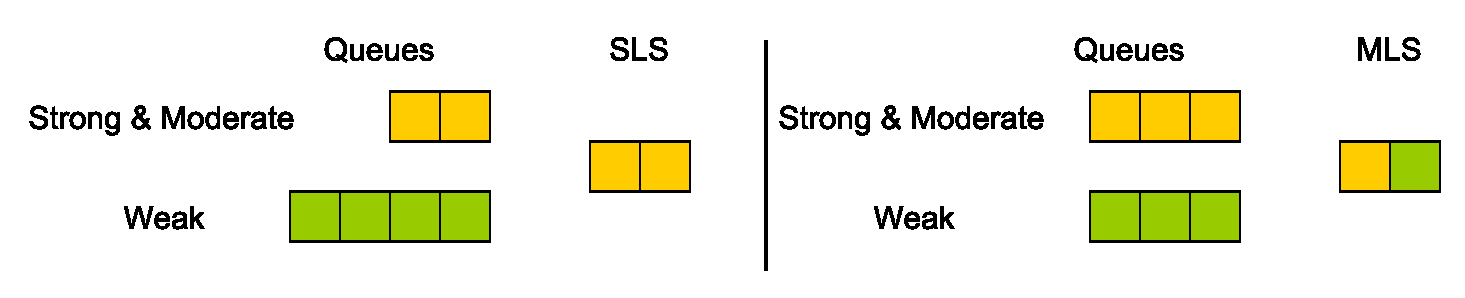
\includegraphics[scale=0.6]{Bilder/sls_mls.pdf}
    	\textsf{\caption{Links ist die Auswahl der auszuführenden Operationen nach SLS-Policy, rechts nach MLS-Policy}}
	\end{center}
\end{figure}

\subsubsection*{Performanzgewinn}
Folgende Abbildung zeigt den Performanzgewinn, der durch die MCC-DB erreicht wird (entnommen aus \cite{LEE}).

\begin{figure}[htb]
	\begin{center}
        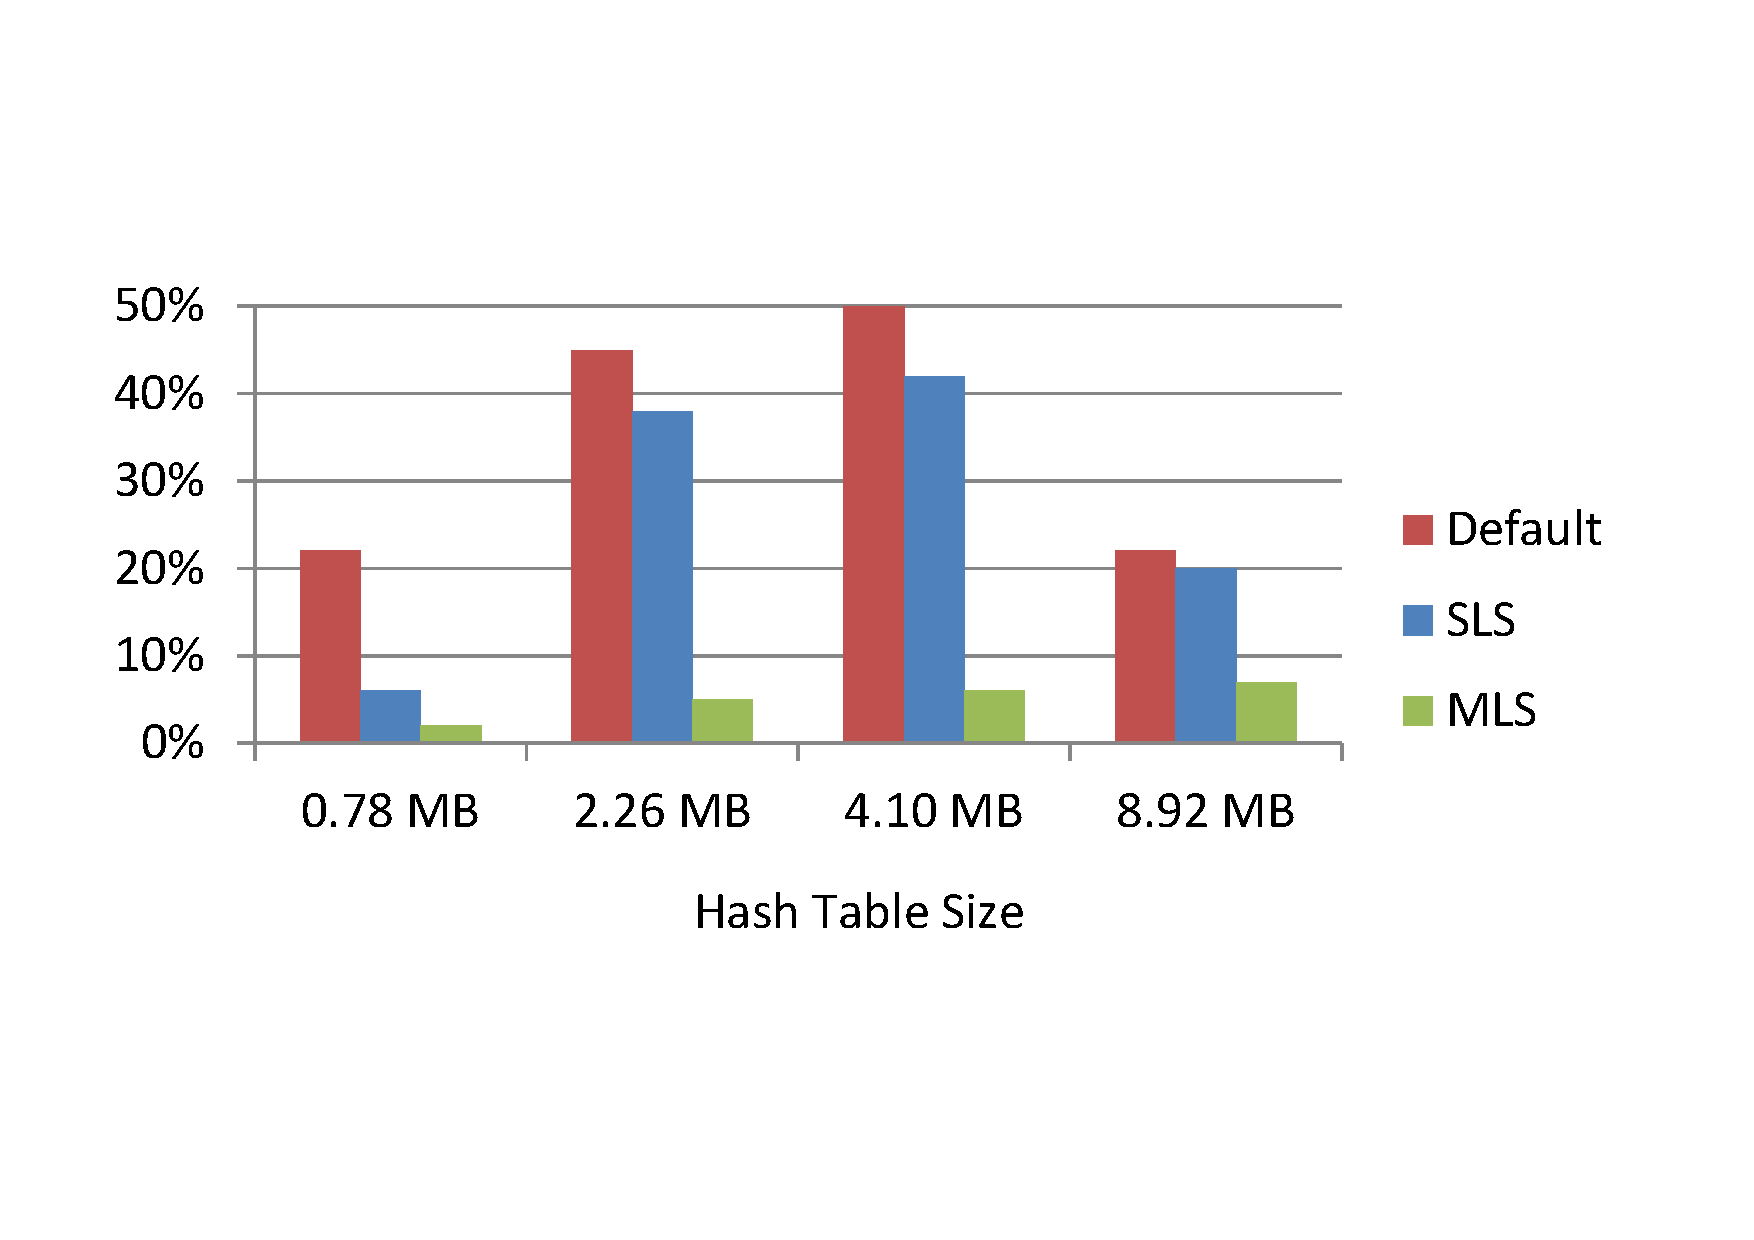
\includegraphics[scale=0.5]{Bilder/mcc_db_chart_cropped.pdf}
    	\textsf{\caption{Performanzverlust in Prozent bei laufenden Queries mit unterschiedlicher Hash-Join-Tabellengröße}}
	\end{center}
\end{figure}

Wir sehen, dass ohne Cache-Partitioning bereits ein Erfolg zu sehen ist. Auf der X-Achse ist der Geschwindigkeitsverlust gekennzeichnet, auf der Y-Achse ist die Größe der Hash-Tabelle der Joins aufgeführt. Während der Effekt bei SLS von der Größe der Hash-Tabelle abhängt, arbeitet MLS mit Cache-Partitioner konstat gut mit einer hohen Effizienz. Weiterhin ist der Effekt bei SLS bei Weitem nicht so groß wie bei MLS.

\section{Parallel SQL Query Auto-Tuning on Multicore}
\label{sec:Parallel-SQL-Query-Auto-Tuning}
\textit{von Tuan-Si Tran}

Der folgende Abschnitt behandelt ein evolutionäres Modell, welches sich mit jeder weiteren Iteration selbstverbessern soll. Dieser Algorithmus basiert auf dem Paper von Pankratius und Heneka \cite{PANKRATIUS}.\\

Datenbanksysteme produzieren Zugriffspläne, die sequentiell abgearbeitet werden. Zur Performanzoptimierung werden zwei Implementierungen vorgenommen. Als erstes wird ein symmetrischer Hash-Join implementiert, der eine parallele Verarbeitung ermöglicht. Bei dem asymmetrischen Hash-Join wird eine Tabelle komplett gehasht und dann jeder einzelne Tupel der anderen Relationen gehasht und auf Gleichheit überprüft. Dadurch muss der zweite Hash-Prozess abwarten, bis der erste mit der Tabelle abgeschlossen hat. In der symmetrischen Implementierung werden beide Relationen parallel vollständig gehasht und dann verglichen. Somit entfällt das Warten auf den anderen Prozess.

\begin{figure}[htb]
	\begin{center}
        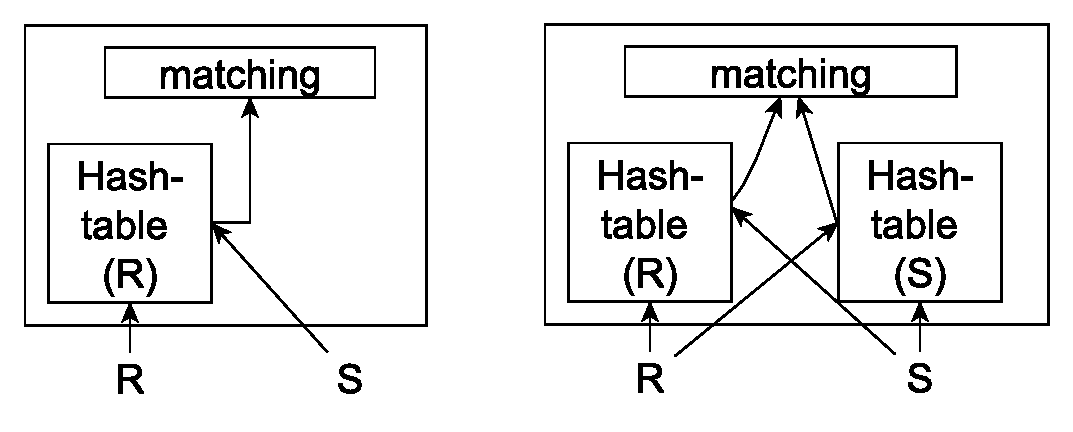
\includegraphics[scale=0.5]{Bilder/s_as_hash_join.pdf}
    	\textsf{\caption{Links ist der asymmetrische und rechts der symmetrische Hash-Join zu sehen}}
	\end{center}
\end{figure}

Die zweite Optimierung ist die Unterteilung der Zugriffspläne in einzelne Abschnitte (Pipeline-Thread), die prinzipiell parallel ausgeführt werden. Diese Unterscheidung wird nach folgendem Algorithmus gemacht. Pankratius und Heneka haben sechs Patterns identifiziert, nach denen Sie den Zugriffsplan unterteilen und verbessern können.

\begin{description}
\item[Pattern 1:] Wenn im Zugriffsplan einen asymmetrischen Hash-Join-Knoten existiert und dieser Knoten als rechtes Kindknoten ebenfalls einen asymmetrischen Hash-Join hat, dann wird zwischen diesen beiden Hash-Joins eine Trennmarkierung für einen Pipeline-Thread eingefügt.
\item[Pattern 2:] Wenn im linken Unterbaum ein Hash-Join-Knoten \texttt{A} existiert, auf dessen Weg zur Wurzel sich ein weiterer asymmetrischer Hash-Join-Knoten \texttt{B} befindet, dann wird zwischen \texttt{A} und seinem Eltern-Knoten eine Trennmarkierung eingefügt
\item[Pattern 3:] Wenn ein Hash-Join Knoten B als direktes Kindknoten im rechten Pfad einen weiteren Hash-Join-Knoten A besitzt und im linken Unterpfad eine große Input-Relation hat und zusätzlich von B zum Wurzelknoten hin noch ein Hash-Join-Knoten gefunden wird, dann wird zwischen B und A eine Trennmarkierung eingefügt.
\item[Pattern 4:] Wenn ein Equi-Join-Knoten identifiziert wird, der sowohl im linken als auch im rechten Kindknoten weitere Bäume hat (also kein Tablescan, Indexscan oder Blatt-Knoten), dann wird der Equi-Join mit dem symmetrischen Hash-Join ersetzt.
\item[Pattern 5:] Wenn ein Equi-Join-Knoten gefunden wird, der als linken Unterpfad einen Baum hat und als rechten Kindknoten ein Blatt-Knoten besitzt, dann wird dieser ebenso mit einem symmetrischen Hash-Join ersetzt
\item[Pattern 6:] Wenn für einen Equi-Join-Knoten das Verhältnis von Relationsgröße des rechten Pfades durch Relationsgröße des linken Pfades größer als 0.9 ist, dann wird auch dieser Knoten mit einem symmetrischen Hash-Join ersetzt.
\end{description}

\begin{figure}[htb]
	\begin{center}
        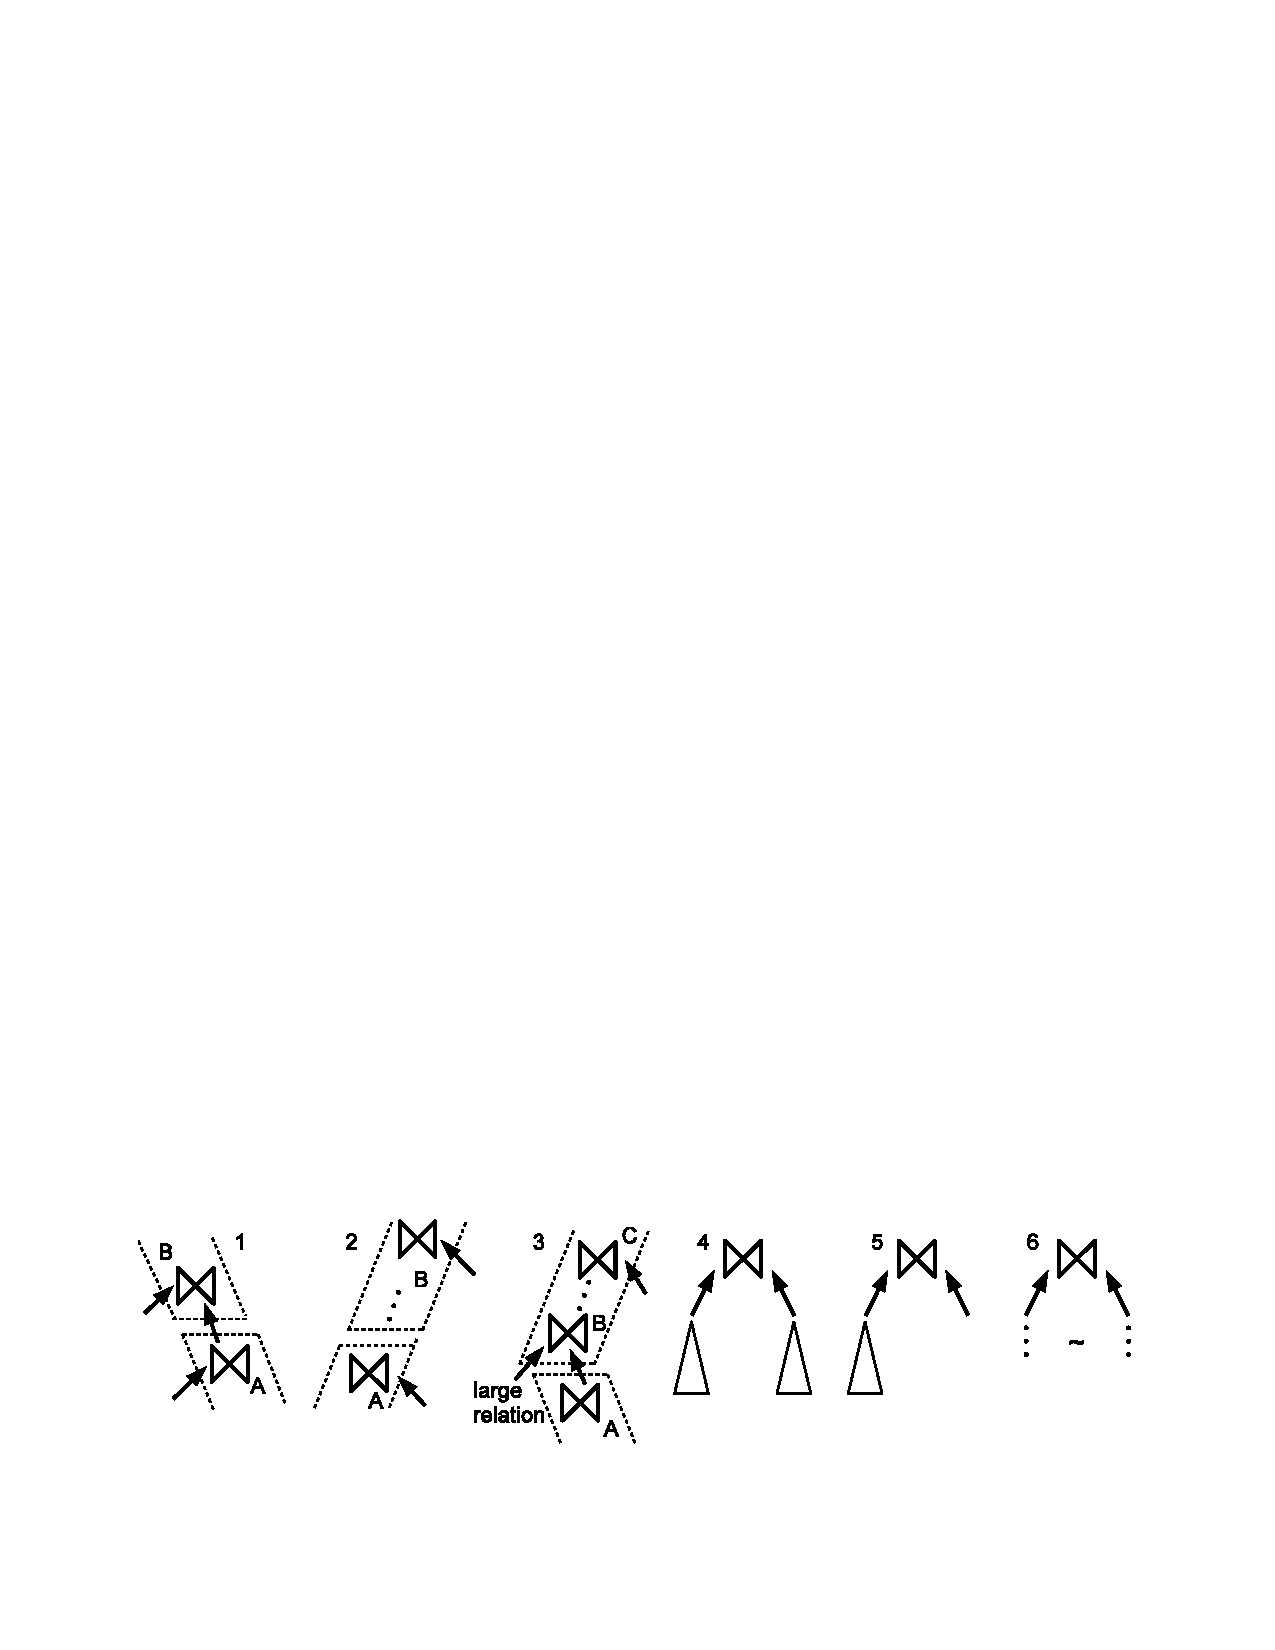
\includegraphics[scale=0.8]{Bilder/patterns_cropped2.pdf}
    	\textsf{\caption{Bildliche Darstellung der Pattern}}
	\end{center}
\end{figure}

Wie bereits erwähnt, ist das Auto-Tuning ein evolutionäres Modell. Dieses Modell setzt darauf, dass Anfragen mehrmals an die Datenbank gesendet werden. Als Beispiel seien hier Applikationen genannt, in denen zum Beispiel mehrere Nutzer die selbe Aktion ausführen können. Bei jeder Iteration wird ein Pattern auf den Zugriffsplan angewendet, welcher in den vorherigen Iterationen noch nicht benutzt worden ist. Dabei wird die tatsächliche Verarbeitungszeit im Log festgehalten. Wenn die Anwendung eines Pattern die Ausführung langsamer machen sollte, wird dieser bei der nächsten Iteration wieder entfernt, ansonsten wird dieser beibehalten. Kann keines der Pattern mehr angewendet werden, versucht die Datenbank zufällig zu optimieren, indem Sie Trennmarkierungen zufällig setzt oder die Buffer-Size zufällig wählt. Auch hier werden die Zeiten mitgeloggt und die Änderungen bei Erfolg beibehalten oder bei Misserfolg verworfen.

\subsubsection*{Performanzgewinn}
Die Fähigkeit, sich in jeder Iteration selbst zu verbessern, ohne dass jemand eingreifen muss, werden von Pankratius und Heneka als Auto-Tuning bezeichnet. Auch der Performanzgewinn kann sich sehen lassen. Vorallem bei größeren Datenmengen werden bis zu 47\% an Performanz gewonnen gegenüber der normalen sequentiellen Ausführung. Allerdings werden in vielen anderen Fällen im Vergleich nur Prozentwerte im einstelligen oder unterem zweistelligen Bereich erreicht. Die ganzen Messreihen sind dem Paper im Anhang detailliert zu entnehmen.

\section{Architecture Aware Hash-Join}
\label{sec:AA-Hash-Join}
\textit{von Christian Dirks}

HashJoin ist eine der entscheidendsten Operationen in Datenbanken. Daher ist es gerade hier wichtig eine Unterstützung von Multicore Rechnern zu erschaffen, um die Leistung noch einmal anheben zu können. Mit steigender Leistungsdifferenz zwischen CPU-Geschwindigkeit und Hauptspeicher muss der HashJoin Algorithmus die Hardware Architektur berücksichtigen, also "architecture aware" werden. Der Architecture Aware Hash Join (AA-Hash Join) \cite{RASHID}\cite{GARCIA} kann sogar durch Software-Prefetching zusätzlich  noch leistungsfähiger gemacht werden. Hier baut der Algorithmus auf vorangegangene Arbeit von Chen et al \cite{CHEN} auf.

AA-Hash Join baut auf dem Model auf, bei dem davon ausgegangen wird, dass mit steigender Anzahl von Festplatten-Armen der Festplattenzugriff kein Bottleneck mehr ist. Tests zeigten, dass bei einem HashJoin die L2 Cache Miss Raten der Größe limitierende Faktor ist. Hier werden durchschnittliche Werte von 29\% bis 69\% Miss-Raten angenommen.

Der AA-Hash Join setzt auf SMT Prozessorarchitekturen. Dabei wird vor allem die Fähigkeit der SMT Prozessoren ausgenutzt zwei parallele Prozesse auf den selben Daten arbeiten zu lassen. Setzt man alleine auf SMT, also nur zwei Prozesse, die sich gegenseitig zuarbeiten, liegen die Daten im L1 Cache des Prozessors. Bei Multicore Prozessoren und mehr als zwei Prozesse liegt diese gemeinsame Datenbasis dann im L2 Cache. Durch diese Prozessorarchitetur entsteht also eine ideale Menge von Prozessen durch : Anzahl CPUs * Anzahl Kerne * Anzahl Prozesse pro Kern. Bei einen Server mit 4 Quadcore CPUs, die SMT unterstützen, ist die ideale Anzahl an Prozessen 32. Dort sind es 4 4-Kern CPUs, was in 16 Kernen resultiert. Durch SMT können jedoch pro Kern 2 parallele Prozesse laufen, was zu den insgesamt 32 Prozessen führt.

Der AA-Hash Join besteht aus drei Phasen. In der ersten Phase werden die Relationen an die Prozesse aufgeteilt und danach geclustert. In der zweiten Phase werden aus den Clustern die Hashtabellen erzeugt und gleichzeitig die Tupelcluster der größeren Relation S erzeugt. Im finalen Schritt werden dann anhand der Hashtabellen die Daten der einzelnen Datencluster durchsucht und in die Tabelle eingetragen.

\subsubsection*{Partitionierung}
\label{sec:AA-Hash-Join_Partitionierung}

Als ersten Schritt werden die Prozesse erzeugt, die vom AA Hash Join verwendet werden. Da sich die Anzahl der verwendeten Prozesse nie ändert, können sie, um Prozessverwaltung zu reduzieren, einmal erzeugt und für den gesamten Algorithmus verwendet werden. Erst wenn der Join komplett ist, werden die Prozesse zerstört. Anschließend werden die Datenstrukturen vorbereitet, um die Indexcluster der kleineren Relation R aufzunehmen. Dafür wird der Indexcluster von R gebildet. Ein einzelner Eintrag im Index besteht aus 4 Byte für den Hash Wert und 4 Byte für den Pointer auf den Tupel, also 8 Byte. Nun müssen entsprechende Cluster erstellt werden, so dass der zur Verfügung stehende Speicher im Cache optimal genutzt wird. Um die Cluster zu erstellen, wird die kleinere R Relation anhand der Anzahl der Prozesse in gleiche Teile aufgeteilt. Jedem Teil wird einer der Prozesse zugewiesen. Die Prozesse gehen sequenziell durch ihre jeweiligen Tupel, was Hardware-Prefetching erlaubt. Jeder Tupel wird anhand seines Schlüssels einem der gebildeten Prozess-spezifischen Cluster zugewiesen, so das jeder Prozess seine Cluster mit Tupeln ähnlicher Schlüssel füllt.

Das bestimmen der Größe der Cluster geschieht anhand spezieller Einschränkungen durch die Größe des verwendeten Caches. Moderne CPUs verfügen über L1 und L2 Cache. L1 Cache ist auf moderneren CPUs zwischen 64 und 256 KByte groß, während L2 Cache normalerweise bis zu 512 KByte groß sein kann. Da das Ziel des Algorithmus ist, möglichst viele Prozesse auf der selben Datenbasis arbeiten zu lassen, muss zuerst zwischen zwei Fällen unterschieden werden. Bei SMT CPU-Architektur  liegen auf einem Kern zwei Prozesse, die jedoch beide parallel auf den L1 Cache zugreifen können. Im Falle einer SMT Singlecore-CPU bedeutet das, dass der gesamte L1 Cache genutzt werden kann um den Indexcluster R\textsubscript{n} aufzunehmen. Schließlich kann zusätzlich der L2 Cache für die Tupel der größeren Relation S verwendet werden. In diesem Fall ist also die Größe des Indexclusters gleich der Größe des L1 Caches.

Gibt es mehr als einen Kern, so sieht das schon anders aus. Bei einem 4-Kern Prozessor beispielsweise gibt es 8 Prozesse, jedoch können über den L1 Cache nur jeweils 2er Pärchen ihre Daten teilen. Daher muss in diesem Fall der Indexcluster im L2 Cache aufgebaut werden. Dadurch wird zwar die Größe des verwendbaren Speichers für den Gesamtalgorithmus beeinflusst und der langsamere L2 Cache wird dem schnelleren L1 vorgezogen. Durch die Parallelität wird dieser Verlust jedoch wieder ausgeglichen. Dennoch muss ein optimaler Wert für den für die Cluster reservierten Speicher gefunden werden. Denn nun müssen sowohl der Indexcluster Rn, also auch die Tupel von R in den Cache passen. Zusätzlich muss Platz bleiben für einige Tupel der S Relation für die spätere Phase der Durchsuchung und auch das Betriebssystem braucht noch Platz für seine eigenen Prozesse. Da die Größe der Hash-Tabelle vor dem Hashen nicht bekannt ist, muss hier eine \textit{Grenze} abgeschätzt werden, der ausreichend Platz bietet. Dies wird in \cite{GARCIA} mit der einfachen Formel: (Größe-R-Relation + Größe-Hashtabelle)/ \textit{Grenze} \textless  Größe-L2-Cache abgeschätzt.

Aber egal ob reiner SMT oder ein Mehrkern-Prozessor vorliegt, die Indextabelle von R wird anhand der Anzahl Prozesse in gleich große Teile zerteilt und an die Prozesse verteilt. Hierbei muss die genaue Struktur der CPU berücksichtigt werden. Bei Intels Quad-Core Architektur beispielsweise teilen sich 2 Kerne ihren L2 Cache. Also können somit 4 Prozesse ihre Hashtabelle teilen. Diese Prozessgruppen erledigen in den kommenden beiden Phasen ihre Arbeiten gemeinsam.

Am Ende dieser Phase ist die R-Relation in gleichgroße Teile aufgeteilt und jede dieser Teile ist in mehrere Cluster ähnlicher Schlüssel gegliedert. Dies ist in Abb. \ref{AAHS_Cluster} dargestellt.

\begin{figure}[htbp]
	\begin{center}
        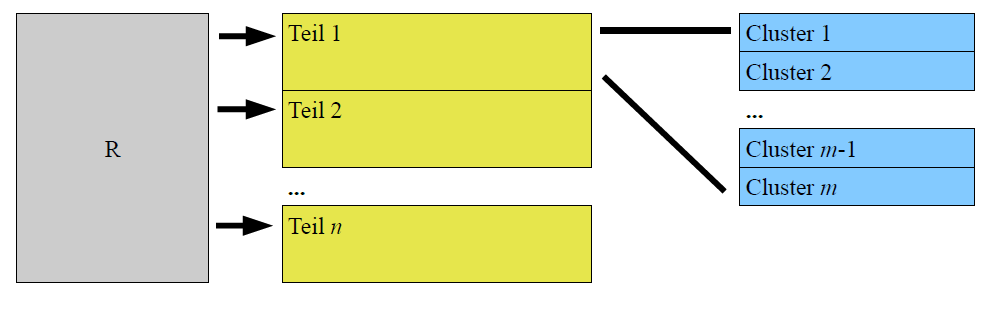
\includegraphics[scale=0.4]{Bilder/Clusterbildung.png}  
    	\textsf{
    		\caption{Die Relation R wird in \textit{n} Teile zerlegt, die wiederum in \textit{m} Cluster ähnlicher Schlüssel zerlegt werden.}
    		\label{AAHS_Cluster}
    		}
		
	\end{center}
	 
\end{figure}

\subsubsection*{Aufbauphase}
\label{sec:AA_Hash-Join_Aufbauphase}

Nachdem sichergestellt ist, dass jeder Prozess seine Arbeit abgeschlossen hat beginnt der nächste Schritt. Um Cache-Miss und Synchronisierungsprobleme zu minimieren, beschäftigt sich jedoch nur der Prozess mit dem kleinsten Prozessindex in der Prozessgruppe mit dem Aufbau der eigentlichen Hashtabelle, während die anderen Prozesse bereits die größere S-Relation clustern. Andere Alternativen sind ineffektiv. Würde beispielsweise jeder Prozess seine eigene Hashtabelle erstellen, so gäbe es mehr Cache Misses, da ein Eintrag nur in einer der Hashtabellen liegt. Arbeiten alle Prozesse an einer Tabelle muss ein Sperrmechanismus her, der die ganze Parallelität zunichtemachen würde, da sie dann aufeinander warten müssten.

Der Prozess, der die Hashtabelle erstellt, nimmt sich jeweils die ersten Cluster der verschiedenen Teile und bildet eine Hastabelle. Dies wiederholt er mit sämtlichen Clustern.

Ähnlich wie in der ersten Phase wird die größere S Relation in Cluster ähnlicher Schlüssel zerlegt. Die gesamte Relation wird in \textit{n} Teile zerlegt, wobei \textit{n} die Anzahl der Prozesse ist. Diese Teile werden nun geclustert wie in der ersten Phase mit der R Relation verfahren wurde. Das heißt, die Teile werden von einem Prozess durchsucht und werden anhand des Schlüssels in Prozess-spezifische Cluster einsortiert. Damit im letzten Schritt jeder Prozess einen Clustersatz hat, muss ein Prozess zwei Teile von S bearbeiten, um dem Hash-Prozess zuzuarbeiten.

Diese Cluster brauchen im Unterschied zu den R-Clustern nicht in den Speicher zu passen. Da die Sequenz der Datenbank bekannt ist, können sie mit einem Prefetch Befehl bereits vorgeladen werden. Auch muss immer nur Platz im Cache für ein paar wenige Tupel aus S sein, da diese durch Prefetching in Schritten geladen werden können.

Am Ende dieser Phase existieren \textit{n} geclusteret Teile von S und \textit{m} Hashtabellen, für jede Gruppe von Clustern gleicher Schlüssel eine. Hier ist \textit{n} die Anzahl der Prozesse und \textit{m} die Anzahl der Cluster. Die Cluster-Anzahl ist abhängig von der Größe des Caches, wie in der ersten Phase beschrieben.

\subsubsection*{Durchsuchphase}
\label{sec:AA_Hash-Join_Durchsuchphase}

Wenn alle Prozesse mit ihrer Arbeit aus der vorherigen Phase fertig sind, beginnen sie ihren zugewiesenen Cluster zu lesen. Um in diesem Schritt die optimale Prozessauslastung zu gewährleisten, aber gleichzeitig Race-Conditions zwischen den Prozessen zu vermeiden, werden die R-Hashtabellen-Cluster Schritt für Schritt geladen. Alle Prozesse arbeiten auf dem selben Hashtabellen-Teil und lesen Schritt für Schritt die Tupel ihrer zugewiesenen S-Relationen aus ihrem Tupelcluster ein und vergleichen sie mit der aktuellen Hashtabelle. Jeder Prozess durchsucht also seine zugewiesenen Tupel und fügt bei Treffer diese in die Buckets der Hashtabelle ein.

Sind alle Prozesse mit ihrem durchsuchen fertig, was im Normalfall die selbe Zeit in Anspruch nehmen sollte, wird der nächste Cluster der Hashtabelle in den Cache eingelesen. Jeder Prozess läd dann den nächsten Cluster der S-Relation und beginnt erneut, die Tupel zu durchsuchen und in die Hashtabellen einzufügen. Dadurch gibt es keine Cache-Misses im Hashtabellen Cluster. Ist es der zweite Fall – also mehrere Hastabellen auf unterschiedlichen L2 Caches eines Multicore Prozessors – müssen diese Tabellen zusätzlich noch zusammengeführt werden, wenn die Hashtabellen gefüllt sind.

Dieser Schritt ist der rechenintensivste des AA-Hash Join Algorithmus. Da der Algorithmus durch seine Strukturierung dafür sorgt, dass die Schlüssel gleichmäßig verteilt sind, leistet Jeder Prozess gleiche Arbeit und kann diese in gleicher Zeit abschließen. Und da jeweils 4 Prozesse auf der selben Hashtabelle arbeiten muss diese nicht immer erneut nachgeladen werden. Die Hashtabelle kann für jeden Teilschritt in dieser Phase im Speicher bleiben und der nächste Teil der Hashtabelle muss auch nur einmal eingelesen werden. Durch den Einsatz von Software-Prefetch-Befehlen kann auch das Laden der Tupel aus den Clustern optimiert werden, so dass die Pipeline bereits die richtigen Daten besitzt und es keine Abbrüche gibt. Hier kann kein Hardware-Prefetching genutzt werden, da die Tupel durch das schlüsselbasierte Clustering nicht mehr sequenziell abgefragt werden können. Da die Software aber die Reihenfolge der Cluster kennt, kann das Hardware-Prefetching durch Software-Prefetching ersetzt werden.

\subsubsection*{Zusammenfassung}
\label{sec:AA_Hash-Join_Zusammenfassung}

Die größere Relation S und die kleinere Relation S werden beide in \textit{n} Teile aufgeteilt. Jeder dieser Teile wird in \textit{m} Cluster zerlegt, so dass \textit{n*m} Cluster pro Relation entstehen, wobei jeder Prozess \textit{m} Cluster besitzt. Eine Hashtabelle besteht aus \textit{n} Clusters – aus jedem Prozess einem – so dass sich die Hashtabelle aus den Clustern ähnlicher Schlüssel bildet.


\subsubsection*{Leistung}
\label{sec:AA_Hash-Join_Leistung}

Die Leistung des Algorithmus ist es also, den Cache möglichst optimal auszunutzen und durch geschicktes Aufteilen Cache-Misses zu reduzieren und Prefetching zu berücksichtigen. In Phasen 1 und 2 kann dies Automatisch durch Hardware-Prefetching geschehen und durch Prefetch-Befehle im Phase 3. Diese optimale Nutzung wird dadurch erreicht, dass die gesamte Arbeit in Portionen zerlegt wird, die in den Cache passen um die Cache-Miss Rate zu reduzieren. Dennoch haben die Tests in \cite{GARCIA} gezeigt, dass die L2-Cache-Miss Rate noch immer das größte Problem darstellt und hier noch über Optimierungen nachgedacht werden kann. Auch die Wahl der richtigen Größe der Partitionen ist entscheidend. Sind diese zu Groß passen sie nicht mehr in den Cache oder lassen keinen Platz mehr für andere Operationen. Sind sie zu klein gibt es jedoch einen Overhead durch die häufigen Kontextwechsel, wenn neue Cluster gelesen werden. Gerade bei einem Prozessor, der mehrere Kerne besitzt ist die Aufteilung wichtig, da hier sowohl Hashtabelle, als auch alles andere im L2 Cache gehalten werden muss, während bei einem SMT-Singlecore die Hashtabellen exklusiv im L1 Cache residieren können. In diesem Fall wird jedoch deutlich, dass das Verfahren die L1 Cache Miss Rate auf ungefähr 2-4 \% Miss-Rate senkt.

Der benötigte Speicher ist gerade bei der Multicore-Variante jedoch nicht zu verachten. Der benötigte Speicher ist das 3,4fache der Größe der Relationen, durch den Overhead der Partitionierung und des Clusterings. Dennoch gibt es einen nicht unerheblichen Leistungsgewinn im Vergleich zu einem Hash Join mit nur einem Prozess. Die Quelle Spricht hier bei einem SMT-Prozessor mit einem Kern von einer Leistungssteigerung um einen Faktor zwischen 2,1 und 2,9 und bei einem Multicore zwischen 2 und 4,9. Diese Teste basieren auf einem Intel Quadcore mit SMT-Unterstützung. Dieser Leistungsgewinn wird Primär durch eine reduzierte L2 Cache-Miss Rate erzielt. Laut den Daten reduziert sich die Miss Rate von 69\% auf 11\%.

\section{Aligned Access-Sort}
\label{sec:Sort_2_AA-Sort}
\textit{von Christian Dirks}

Sortieren ist einer der wichtigen Datenbankoperationen, doch bisherige Sortierverfahren sind nur begrenzt für Multithread-Anwendungen geeignet. Der bevorzugte \textit{quicksort} zieht kaum Vorteile aus mehreren Pozessoren. Aligned-Access Sort \cite{INOUE} setzt hier auf eine andere Basis. Aligned-Access- Sort (AA-Sort) ist ein Sortieralgorithmus der sowohl Single Instruction Multiple Data (SIMD) Befehle nutzt als auch Parallelität auf Prozessebene. Er ist für die Verwendung auf Prozessoren mit geteiltem Speicher entwickelt und zielt auf die Optimierung der SIMD Befehle um optimalen Zugriff auf den Speicher zu ermöglichen.

SIMD Befehle wie beispielsweise SSE oder VMX haben 128-Bit Platz für Daten neben den Registern und dem eigentlichen Befehl. Doch um diesen Vorteil effektiv nutzen zu können muss dieser Datenplatz effizient genutzt werden, die zu sortierenden Daten also idealerweise in diesen 128-Bit Platz passen ohne zu viele Bits unbenutzt zu lassen. So kann ein einfacher Vergleich mehrerer Werte in einem Befehl ausgeführt werden, ohne das die Werte nachgeladen werden müssen. Alle Werte werden in den Datenbereich des SIMD Befehls gespeichert und der Vergleich greift nun nicht mehr auf den Speicher, sondern nur noch auf den Datenbereich des Befehls zurück.

Um diese Besonderheit in einen Vorteil zu verwandeln setzt AA-Sort auf zwei Schritte in der Sortierung. Der spezielle in-core Sortierungsschritt setzt auf SIMD Befehle um Speicherzugriff und Pipeline optimal zu nutzen. Kernidee hierfür ist \textit{combsort} \cite{LACEY} zu optimieren, so dass er auf Blockebene und nicht mehr auf Elementebene anwendbar ist, wodurch die SIMD Unterstützung verbessert wird.

Dies macht jedoch einen zweiten Schritt – die out-of-core Sortierung – erforderlich. Denn dafür müssen die Daten in eine ideale Form gebracht werden. Diese lassen sich dann mit einem \textit{mergesort} Ansatz im in-core Teil sortiert.

Der gesamte AA-Sort zerlegt die Daten zuerst in Blöcke, die in de L2 Cache des Prozessors passen. Der in-core Sortieralgorithmus sortiert diese Blöcke. Die sortierten Blöcke werden schließlich durch den out-of-core Algorithmus zusammengeführt. Beide Algorithmusphasen profitieren von der Parallelität mehrerer Prozesse.


\subsubsection*{Blockbildung}
\label{sec:AA-Sort_Blockbildung}

Die Größe der Blöcke hängt von den zu sortierenden Daten ab. SIMD Befehle haben 128 Bit Datenplatz. Die Blöcke müssen daher so aufgeteilt werden, dass sie in diesen Platz passen. Im Falle von 32 Bit Integer wäre das Blocke von jeweils 4 Integerwerten. Aber auch andere Größen sind denkbar, solange sie sich effektiv auf die 128 Bit aufteilen lassen. Es entstehen Vektoren die jeweils die Daten der Blöcke beinhalten. Im Beispiel der 32 Bit Werte, die in der weiteren Beschreibung des Algorithmus zugrunde gelegt werden, entstehen \textit{n} = N/4 Vektoren, also \textit{n} Vektoren, die jeweils 4 Elemente der gesamten N Werte beinhalten.

Aber auch der Cache kann bei der Aufteilung eine Rolle spielen. Passt ein Block nicht in den Cache eines Prozessorkerns muss eine insgesamt kleinere Blockgröße angestrebt werden, auch wenn das zur Folge hat, dass der SIMD-Datenteil dann nicht optimal gefüllt ist.

\subsubsection*{In-core Algorithmus}
\label{sec:AA-Sort_In_Core}

Der in-core Algorithmus baut auf \textit{combsort} auf, was wiederum eine Erweiterung von \textit{bubblesort} ist. \textit{Bubblesort} vergleicht zwei benachbarte Elemente und tauscht sie wenn nötig. \textit{Combsort} geht einen Schritt weiter und vergleicht nicht mehr nur noch benachbarte Elemente. Er beginnt das Vergleichen mit weit auseinanderliegenden Elementen. Diese Distanz, auch \textit{Gap} genant wird bei jedem Schritt durch den empirischen Faktor 1,3 dividiert. So reduziert sich mit jedem Schritt die Distanz.

Es gibt jedoch Probleme die die Verwendung von SIMD im Zusammenhang mit \textit{combsort} erschweren. Durch die wiederholende Division durch 1,3 entstehen \textit{Gaps}, die keine Vielfachen der Blockaufteilung sind. Dadurch kommt es zu unregelmäßigen Zugriffen auf die Blöcke. Aber auch \textit{Gaps} kleiner als die Schrittweite der Blocke erzeugt Probleme. In diesem Fall kann die Datenparallelität nicht mehr ausgenutzt werden, da ein Block und somit ein Prozess unregelmäßig zugegriffen wird.

Um diese Probleme des \textit{combsorts} zu umgehen und SIMD zu verwenden, setzt der in-core Algorithmus auf 3 Schritte.


(1) Jeder Block wird in aufsteigender Reihenfolge sortiert

(2) \textit{Combsort} wird verwendet um die Elemente der Blöcke in die \textit{Vertauschte Form} zu bringen.

(3) Die \textit{Vertauschte Form} wird wieder in die Originalform überführt


Durch diese Schritte wird ein \textit{combsort}-ähnliches Verhalten erzeugt, das jedoch nur \textit{Gaps} von Vielfachen der Blockaufteilung besitzt. Der erste Schritt(siehe Abb. \ref{AAS_Block}) entspricht dem \textit{combsort} mit den \textit{Gaps} N/n, N/n*2, N/n*3, wobei n die Anzahl Elemente pro Block ist und N die Anzahl aller Elemente. Diese Sortierung lässt sich mit Vectorbefehlen aus dem SIMD Befehlssatz problemlos und ohne viel Rechenaufwand lösen da die Blöcke ja bereits in passender 128 Bit Größe vorliegen.

Der zweite Schritt tauscht nun die Elemente zwischen den einzelnen Blocken in die Vertauschte Form(siehe Abb. \ref{AAS_Block}). Dafür wird der combsort-Algorithmus nun nicht für einzelne Elemente, sondern auf Blockebene durchgeführt. Jeder Vergleich zweier Blöcke (hier A und B) besteht dabei aus zwei Teilen. Zuerst werden alle Elemente aus A mit den korrespondierenden Elementen aus B vertauscht, so das die kleineren Werte in A stehen. Dann wird das Selbe erneut durchgeführt. Diesmal werden jedoch die ersten 1 bis \textit{n}-1 Werte aus A mit den Werte 2 bis \textit{n} aus B verglichen. Diese beiden Schritte sind in Abb. \ref{AAS_Vectorswap} zu sehen. Dies ersetzt zwar die innere Schleife des \textit{combsort} durch zwei Schleifen, jedoch können nun die Vergleiche auf Basis der SIMD Vectorbefehle ausgeführt werden. Der dritte Schritt sortiert die einzelnen Blöcke erneut, aufsteigend(siehe Abb. \ref{AAS_Transposed_Order}).

Durch dieses Herangehen werden die beiden angesprochenen Probleme der \textit{Gap}-Bildung von zu Kleinen oder nicht Vielfachen der Blockaufteilung vermieden. Teile der combsort-Schleifen werden einfach auf andere Operationen abgebildet. Die verbleibende Schleife kann dann mit dem Selben Schema und der Division durch 1,3 auf der Ebene der Blöcke durchgeführt werden. Insgesamt hat der in-core Algorithmus eine Laufzeit von O(n log( n) ) im Durchschnitt und O(n\textsuperscript{2}) im schlechtesten Fall. Der große Vorteil gegenüber anderen Sortierverfahren, die auch im schlechtesten Fall O(n log(n) ) erreichen, ist die Verwendung von SIMD Befehlen, so das Zugriffe auf den Speicher reduziert und Cache-Misses vermieden werden. Die benötigten Werte werden bereits im 128 Bit-Datenteil mitgeliefert und müssen nicht mehr separat aus dem Speicher geladen werden. Dadurch ist dieses Verfahren deutlich schneller. Dennoch ist die Sortierung nicht abgeschlossen, es wurde nur eine Blockaufteilung erzeugt, die einem bekannten Schema folgt. Die finale Sortierung wird im nächsten Algorithmusteil, dem  out-of-core Algorithmus durchgeführt.


\begin{figure}[htbp]
	\begin{center}
        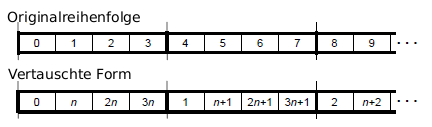
\includegraphics[scale=0.5]{Bilder/AAS_Vor_Sortierung.png}  
    	\textsf{
    		\caption{Die zu sortierenden Daten werden in 128-Bit Blöcke zerlegt, sortiert und in die \textit{Vertauschte Form} gebracht.}
    		\label{AAS_Block}
    		}
	\end{center}
\end{figure}

\begin{figure}[htbp]
	\begin{center}
        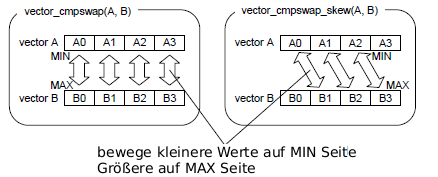
\includegraphics[scale=0.5]{Bilder/AAS_Vectorvertauschung.png}  
    	\textsf{
    		\caption{Diese beiden Vertauschungsschritte sind leicht mit SIMD Befehlen umzusetzen und erlauben es den \textit{combsort} auf Blockebene anzuwenden.}
    		\label{AAS_Vectorswap}
    		}
	\end{center}
\end{figure}

\begin{figure}[htbp]
	\begin{center}
        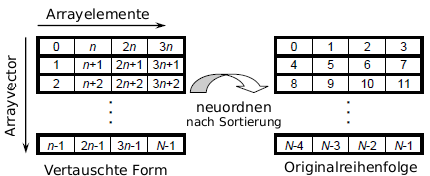
\includegraphics[scale=0.5]{Bilder/AAS_Nach_Sortierung.png}  
    	\textsf{
    		\caption{Die sortierte \textit{Vertauschte Form}(links) wird wieder zurückgeführt in die originale Aufteilung(rechts). Die Rückführung geschieht im in-core Algorithmus.}
    		\label{AAS_Transposed_Order}
    		}
	\end{center}
\end{figure}


\subsubsection*{Out-of-core Algorithmus}
\label{sec:AA-Sort_Out_Of_Core}

Am Ende des in-core Schrittes ist jeder Block in sich selbst sortiert und existiert in der bekannten Struktur der Vertauschten Form. Der out-of-core Algorithmus sortiert nun die Blöcke zurück in eine zusammenhängende Form(siehe Abb.\ref{AAS_Transposed_Order}). Auch diese Sortierung setzt auf den SIMD Befehlssatz. Hier wird jedoch auf einen \textit{mergesort} zurückgegriffen, wie in Abb. \ref{AAS_Mergesort} gezeigt. Zwei Blöcke mit P Elementen lassen sich dabei in log(P) +1 Schritten sortieren. Jeder Schritt führt nur einen Vectorvergleich, zwei Vectorauswahlen und ein bis zwei Vectorvertauschungen aus. Da die \textit{Vertauschte Form}, in denen die Elemente vorsortiert sind bekannt ist, kann dieses Wissen genutzt werden. Dadurch reduziert sich die Anzahl der bedingten Verzweigungen im Quellcode auf eine Verzweigung pro P Elemente aufgrund ihrer Blockform. Ohne dieses Vorarbeit wäre es eine Verzweigung pro Element und nicht nur pro Block. Da jede Verzweigung potenziell ist mit einem Pipeline-Abbruch gleichgesetzt werden kann, ist der vorgestellte Algorithmus durch die Vertauschte Form performanter. Die Laufzeit des out-of-core Algorithmus ist O(n).

\begin{figure}[htbp]
	\begin{center}
        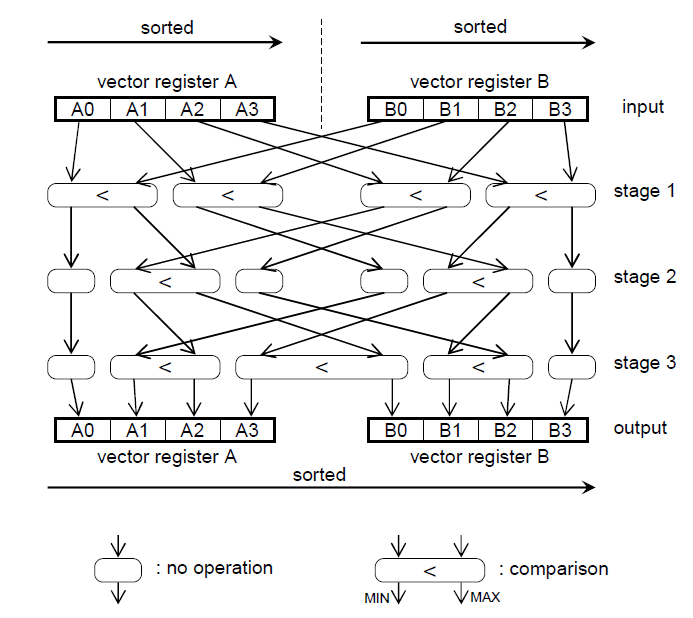
\includegraphics[scale=0.5]{Bilder/mergesort_variant.png}  
    	\textsf{
    		\caption{Wissen über die Struktur der \textit{Vertauschte Form} erlaubt es, zwei Blöcke mit \textit{mergesort} in wenigen SIMD Vectoroperationen zu sortieren.}
    		\label{AAS_Mergesort}
    		}
	\end{center}
\end{figure}

\subsubsection*{Zusammenfassung}
\label{sec:AA-Sort_Zusammenfassung}

Der gesamte AA-Sort teilt sich in drei Phasen. In der ersten werden die zu sortierenden Daten in 128 Bit Blöcke aufgeteilt, um in den Datenteil der SIMD Befehle zu passen. Diese unabhängigen Blöcke werden nun durch den in-core Algorithmus parallel von mehreren Prozessen sortiert. Dieser Schritt basiert auf einer \textit{combsort}-ähnlichen Sortierung, wobei durch geschickte Aufteilung auf Blockebene \textit{combsort}-Schleifen mit unpassendem \textit{Gap} auf zusätzlich SIMD Befehle abgebildet werden. Anschließend werden die Blöcke parallel von mehreren Prozesse durch einen \textit{mergesort} zusammengesetzt. Dieser \textit{mergesort} im out-of-core Algorithmus nutzt Wissen über die Struktur der Blöcke um Pipeline-Abbrüche zu reduzieren. Sowohl in-core, als out-of-core Algorithmus setzten auf den SIMD Befehlssatz, um Cache-Miss-Raten zu reduzieren, indem sie die zu betrachtenden Daten bereits mitliefern.

In Bezug zu Datenbankanwendungen könne die zu sortierenden Werte beispielsweise Paare aus {key, data} sein. Hier muss jedoch abhängig von den verwendeten Daten der AA-Sort angepasst werden. Unter Zuhilfenahme des \textit{radixsort} lassen sich dann auch größere Daten wie beispielsweise 64-bit Integer und 10-Byte ASCII Strings sortieren. Dafür wird aus den Datenelementen die ersten paar Bytes extrahiert und in 32-Bit Integer codiert. Ab hier kann normal weiter sortiert werden, solange keine zwei gleichen 32-Bit Schlüssel auftauchen. In solchen Fällen müssen dann auch die restlichen Bytes betrachtet werden, um korrekt zu sortieren. Dadurch wird der AA-Sort um den Faktor 1.6 langsamer ist jedoch noch immer um den Faktor 5 schneller als vergleichbare Sortieralgorithmen (GPUTeraSort \cite{GOVINDARAJU}).

\subsubsection*{Leistung}
\label{sec:AA-Sort_Leistung}

Der große Vorteil des AA-Sort ist die Vermeidung von Pipeline-Abrissen und die Aufteilung der Arbeit auf mehrere Prozesse. Die Authoren \cite{INOUE} geben die Komplexität mir O(n log(n) ) an, auch im schlimmsten Fall. Da jedoch Parallelität ausgenutzt werden kann, kann dies auch mit O(n log(n) / \textit{k}) angeben werden, wobei \textit{k} für die Anzahl der Prozesse steht. Jedoch darf hier \textit{k} nicht größer als die Anzahl der Blöcke sein. 

Bei großen Datenmengen von 32 Bit Integerwerten von insgesamt 128 Mio. Elementen (512 MB) ist AA-Sort um den Faktor 3 schneller als vergleichbare Sortierverfahren aus der STL. Jedoch ist aufgrund der heuristischen Herangehensweise denkbar, dass der in-core Teil für einige nicht ideal-große Start-Datensätze reduzierte Leistungen erzielt. Der out-of-core Teil ist in seiner Leistung jedoch weitestgehend unabhängig von der Größe und der Art der Daten.

Die Spezialisierung auf SIMD Befehle bedeutet jedoch, dass die Leistung ohne entsprechende Prozessorarchitekture drastisch sinkt. Der in-core Algorithmus wird dadurch um den Faktor 7,47 langsamer und der out-of-core Teil um 3,33. Hier wird noch einmal deutlich, dass SIMD gerade im in-core Teil das größte Verbesserungspotenzial mit sich bringt.

\section{Evaluation}
\label{sec:Evaluation}
In diesem Abschnitt betrachten wir noch einmal zusammenfassend die Algorithmen und betrachten den Aufwand und Nutzen.
Die MCC-DB erreicht sehr gute Ergebnisse, sofern der Cache-Partitioner angewendet wird. Mit der MLS-Strategy kann der Performanzverlust minimal gehalten werden. Allerdings wird dazu die Hilfe des Betriebssystems benötigt. Der Cache-Partitioner funktioniert nur, wenn das OS auch abgepasst worden ist. Der Algorithmus errechnet aufgrund statischer Analysen die Optionen zur Optimierung und wendet diese mit Hilfe des Betriebssystems an.

Parallel SQL Query Auto-Tuning on Multicore hingegen arbeitet lediglich mit Optimierungen am Zugriffsplan, weswegen der initiale Aufwand geringer ausfällt. Hinzu kommt, dass der Algorithmus in der Lage ist, sich selbstständig zu verbessern. In mehreren Iterationen wird versucht nach bestimmten Mustern die Verarbeitung zu verbessern. Dabei ist der Algorithmus nicht vom Betriebssystem abhängig. Weiterhin ist dieser sehr flexibel und es lassen sich prinzipiell mehr Querys erreichen als mit MCC-DB. Der Optimierungseffekt fällt dabei aber im Normalfall geringer aus als bei MCC-DB, da die Optimierung auf höherer Ebene stattfindet als bei der MCC-DB.

Architecture Aware Hash-Join ist eine reine Optimierung des Hash-Joins, einem der rechenintensiven Datenbankoperationen. Der Algorithmus ist auf eine spezielle Architektur angewiesen, Intels SMT-Prozessoren. Durch geschickte Cache-Nutzung in Kombination mit der Parallelität kann die Leistung des Hash-Joins erheblich verbessert werden. 8 Prozesse beschleunigen den Join um einen Faktor zwischen 2 und 4,9. 

Alligned Access Sort ist ein reiner Sortieralgorithmus und daher nicht nur an Datenbankanwendungen gebunden. Ähnlich wie bei dem AA-Hash Join ist das Ziel eine geschickte Cache-Nutzung und paralleler Verarbeitung. Dabei setzt er auf bekannten Sortierverfahren auf, optimiert diese jedoch so, dass er um einen Faktor von 3 schneller ist als andere Sortieralgorithmen. AA-Sort baut auf SIMD-Prozessorbefehlen auf, die jedoch von allen moderneren Prozessoren unterstützt werden. Da AA-Sorts finale Leistung von den zu sortierenden Daten abhängt muss der genaue Leistungsgewinn bei Datenbank-Systemen jedoch noch in der Praxis erprobt werden.
\chapter{Zusammenfassung und Ausblick}
\label{sec:Zusammenfassung-Ausblick}

\section{Zusammenfassung}
\label{sec:Zusammenfassung}

Durch den Paradigmenwechsel von immer schnelleren Prozessoren hin zu Multicore-Prozessoren greifen die bisherigen Optimierungen nur noch begrenzt. Daher müssen neue Ideen und Algorithmen umgesetzt werden, damit Datenbank-Systeme mit den steigenden Anforderungen schritthalten können. Dies erfordert einen neuen Umgang mit Zugriffen auf den Hauptspeicher und den Cache. Aber auch die Planung der Prozessor-Pipeline und der Prozessverteilung wird immer wichtiger.

Um diese Optimierung durchzuführen können einerseits einzelne Teilbereiche und Datenbankoperationen einzeln optimiert werden, wie es beim AA-Sort und AA-Hash Join der Fall ist. Diese beiden Algorithmen versuchen für eine konkrete Aufgabenstellung Zugriffe auf den Cache so zu optimieren, dass paralleler Zugriff optimal möglich ist, ohne zu viele Cache-Miss und Pipeline-Abbrüche zu erzeugen. Dadurch können sie ihren Aufgabenbereich deutlich beschleunigen.

Andererseits kann die Optimierung auch globaler betrachtet werden. Beim Minimizing Cache Conficts Ansatz geht es darum, den Cache optimal zu verwalten. Datenbankoperationen werden anhand ihres Cache Bedarfs eingeteilt um sie anhand dieses Kriteriums optimal zu verteilen und zu bearbeiten. Dies geschieht um einen Zugriffsplan. Beim Auto-Tuning geht es ebenfalls um die Optimierung des Zugriffsplans. Hier wird jedoch auf ein evolutionäres System gesetzt, dass sich selbst optimieren kann. Wiederkehrende Anfragen werden systematisch mit unterschiedlichen Pattern und Cachezuweisungen aufgerufen und die so gewonnenen Daten werden für die automatische Optimierung herangezogen. Dabei werden auch Teile des Zugriffsplans auf unterschiedliche Prozesse verteilt, wodurch auch eine ideale Prozessaufteilung entsteht.

Beide Herangehensweise können signifikante Leistungssteigerungen erzeugen, so das davon auszugehen ist, dass in Zukunft Datenbanksysteme auf einige, oder - wenn möglich - mehrere dieser Optimierungen einsetzen werden.


\section{Andere Ansätze}
\label{sec:AndereAnsatze}
Die in dieser Ausarbeitung im Detail vorgestellten Algorithmen sind nur ein Teil der Möglichkeiten, mehrere Prozesse für Datenbankabfrage-Optimierung zu nutzen. Um einen kleinen Blick auf diese anderen Ansätze zu werfen, werden im folgenden einige der Interessanteren betrachtet. Es gibt jedoch zusätzlich noch weitere Ansätze und Algorithmen, die hier nicht mehr erwähnt werden. Die meisten Dieser ähneln jedoch denen im Detail vorgestellten Algorithmen indem sich versuchen, die Zugriffe auf den Speicher zu optimieren und Cache-Misses und Pipeline-Abbrüche zu reduzieren.

\subsection{Netzwerkprozessor}
\label{sec:Netzwerkprozessor}

Ein Ansatz mehrere Prozesse optimaler zu unterstützen ist es, spezielle Prozessoren zu verwenden, die besser geeignet sind mit einer großen Anzahl von Prozessen umzugehen. \cite{GOLD} Netzwerkprozessoren sind spezielle Prozessoren die sich durch eine auf Prozesse spezialisierte Architektur auszeichnen. Pro Prozessorkern – Microengine genannt – können bis zu 8 Prozesse parallel arbeiten und durch spezielle Register und Cache kann ein Kontextwechsel ohne großen Overhead in einem einzelnen Prozessorzyklus durchgeführt werden.

Durch die spezielle Art der Hardware wird jedoch der Programmieraufwand größer. Viele automatisierte Vorgänge müssen durch das Programm selber durchgeführt werden. Ein Prozesswechsel muss explizit angegeben werden und der nächste Prozess wird nach dem Round-Robin Verfahren ausgewählt. Der Prefetcher muss ebenfalls vom Programmierer selber festgelegt werden. Dadurch kann kontrolliert werden, dass kritische Daten auch wirklich immer im Speicher liegen und nicht erst nach einem Cache-Miss neu geladen werden müssen. Andere Daten können explizit im RAM belassen werden.

Ein Sequenzieller Scan einer Tabelle einer Datenbank kann beispielsweise so aufgeteilt werden, dass eine Page pro Microengine durchsucht wird. Die 8 Prozesse der Microengine bearbeiten jeweils einen Eintrag. Dafür wird die Page explizit in den Cache der Microengine geladen.

Da Netzwerkprozessoren nur über wenig zusammenhängendem Cache verfügt, besteht gerade beim HashJoin die Gefahr, dass die Buckets zu groß werden. Da ihre Größe nicht effektiv vorhergesehen werden kann muss die Hashtabelle sicherheitshalber im RAM belassen werden. Es entsteht ein größerer Overhead beim Zugriff auf die Tabellen. Aber durch die parallele Bearbeitung der Pages gibt es dennoch einen zeitlichen Gewinn.

Die Verwendung eines Netzwerkprozessors ist aufgrund des umfangreicheren Programmieraufwandes nicht einfach, kann aber mit anderen Optimierungen und Algorithmen zusammen verwendet werden. Vermutlich lassen sich die in dieser Ausarbeitung vorgestellten Algorithmen und Ansätze auch auf einen Netzwerkprozessor übertragen, in manchen Fällen vielleicht sogar effektiver als auf einem herkömmlichen Prozessor.


\subsection{CUDA}
\label{sec:CUDA}

Im Vergleich zu CPUs besitzen die meisten modernen GPUs (Grafikprozessoren) eine ca 10x höhere Rechenleistung und 10x größere Speicherbandbreite. Zusätzlich sind sie bereits für Multiprozess-Tätigkeiten optimiert, bieten schnelle Kommunikation zwischen Prozessen und erlauben zufälligen Zugriff auf Speicheradressen. Dies wird durch on-chip Speicher erreicht, der zusätzlich zum schnellen Grafikspeicher verwendet wird. All dies sind Eigenschaften, die bei einer Multiprozess-Datenbank erwünscht sind. Problem ist hier jedoch, dass die Kommunikation zwischen CPU und GPU über den BUS abläuft mit begrenzte Bandbreite abläuft. Effektiver RAM- und Festplattenzugriff ist daher unmöglich. Das reduziert den Nutzen auf Operationen mit einer festen Datenmenge. Die Daten müssen einmalig auf die GPU übertragen werden und können dort gehalten werden.

Über die Programmiersprache CUDA kann die GPU programmiert werden und das nicht nur für grafische Anwendungen. So kann die GPU in einen Coprozessor verwandelt werden, der Relationsanfragen bearbeiten kann und Arbeitskraft der CPU für andere Speicherzugriffs-lastige Aufgaben freimacht. \cite{HE} Optimierte Algorithmen sind jedoch erforderlich, um den Nachteil der Bustransferrate auszugleichen. Pro GPU-Prozessorkern laufen ganze Prozessgruppen. SIMD Unterstützung und Architektur sind einem Netzwerkprozessor nicht unähnlich. Das in [Quelle] erstellte System setzt einen Abschätzungsmechanismus ein, um Aufgaben, die Idealerweise auf der GPU verarbeitet werden könne, an diese weiterzugeben. Hierbei wird die Bus-Transferrate mit berücksichtigt um einen Leistungsgewinn zu erzielen. Durch die Bus-Limitierung ist es erforderlich, die kommunizierten Daten genau zu planen. Sämtliche Anweisungen und Daten, alle Tupel und Indexe werden an die GPU übertragen. Bei Abschluss der Arbeit wird ausschließlich das Endprodukt zurückgeliefert. Es lassen sich ausschließlich read-only Datenbankoperationen durchführen. Änderungen können durch den GPU Coprozessor nicht in akzeptabler Zeit realisiert werden.

Somit ist der Einsatz der GPU eher als Unterstützung zu sehen. Sie erlaubt es, der CPU Arbeit abzunehmen und CUDA kann somit parallel zu den anderen hier vorgestellten Algorithmen und Ansätzen zur Leistungssteigerung einer Datenbankanwendung eingesetzt werden.


\subsection{Mehrere Datenbank-Engines}
\label{sec:DBEngines}

Ein Ansatz der Optimierung von Datenbanken an ein Multicore-System ist es, die Hardware als ein verteiltes System zu behandeln. In diesem Sinne wird nicht die Behandlung einer Datenbankanfrage auf die Prozesse verteilt, sondern die Datenbank selber. Somit gibt es mehrere Datenbankengines, die auf dem selben Rechner laufen. Das bedeutet, dass nur noch eine Middleware-Schicht entwickelt werden muss, die die Anfragen auf die verteilte Datenbank-Engines vermittelt.

\textit{Multimed} \cite{SALOMIE} ist das Konzept einer derartigen Datenbank-Engine. Es setzt dabei auf eine Master-Datenbank und mehrere Satelliten-Datenbanken. Vorteilhaft ist eine leichte Skalierbarkeit, da sich mit steigenden Prozessorkern-Anzahl einfach die Anzahl der Satelliten erhöht werden kann. Das bereits existierende Know-How verteilter Datenbanken kann eingesetzt werden. Nach außen hin tritt \textit{Multimed} wie eine einzelne Datenbankengien auf. Updates werden auf der Master-Datenbank durchgeführt und asynchron an die Satelliten weitergegeben. Datenbankanfragen die kein Update erfordern, werden hingegen von den Satelliten durchgeführt. 

Zwar wird durch diesen Ansatz die Menge an Speicher pro Datenbank limitiert, jedoch sagen die Autoren des Papers \cite{SALOMIE}, das der Ansatz mehrere Datenbanken mit einem Teilspeicher schneller sei, als eine herkömmliche Datenbank, die über den gesamten Speicher verfügt.

\appendix
\input{Anhang}
\newpage

\nocite{*} % Auch nicht zitierte Literatur auff�hren

% Literaturverzeichnis soll im Inhaltsverzeichnis auftauchen
\clearpage
\phantomsection % Hyperlink vom Inhaltsverzeichnis zum Literaturverzeichnis
\addcontentsline{toc}{chapter}{Literaturverzeichnis}
% Literaturverzeichnis anzeigen
\bibliography{literatur}

\end{document}

